% !TEX root = lectnote.tex
% !TEX spellcheck = en_GB-oed 

\chapter{Recurrence sequences}\label{Recurrence sequences}
In this chapter we consider an important mathematical tool, the so-called recurrence.
It is a very useful problem solving strategy that solves a problem by reducing it 
to smaller instances of the same problem.
\section{Examples of recurrence relations}
To compute $n!$ by using recurrence we rewrite it as follows
$$
n!=\prod_{k=1}^n k=n\cdot\prod_{k=1}^{n-1} k=n\cdot (n-1)!.
$$
That is, we have the definition
\begin{equation*}
n!=
\begin{cases}
1 & \mbox{ if }n=1,\\
n\cdot(n-1)! & \mbox{ if }n>1.
\end{cases}
\end{equation*}
To compute 4! one has to evaluate $4\cdot(4-1)!$, so it remains to compute 3!,
applying the recurrence relation again it follows that $4!=4\cdot 3\cdot(3-1)!$.
At the end we get that $4!=4\cdot 3\cdot 2\cdot 1$. Of course it is not an efficient
way to compute $n!$, but recurrence helps to understand and to analyze problems.

Binomial coefficients can be defined via recurrence. The main idea is to use the 
well-known identity
$$
\binom{n}{k}=\binom{n-1}{k}+\binom{n-1}{k-1}.
$$
The recursive definition goes as follows
\begin{equation*}
\binom{n}{k}=
\begin{cases}
1 & \mbox{ if }k=0\mbox{ or }k=n\\
\binom{n-1}{k}+\binom{n-1}{k-1} & \mbox{ if }n>k>0.
\end{cases}
\end{equation*}
We apply the above definition to compute $\binom{5}{3}:$
$$
\binom{5}{3}=\binom{4}{3}+\binom{4}{2}.
$$
We only need to determine $\binom{4}{3}$ and $\binom{4}{2}$.
\begin{align*}
\binom{4}{3}&=\binom{3}{3}+\binom{3}{2}\\
\binom{4}{2}&=\binom{3}{2}+\binom{3}{1}.
\end{align*}
Since by definition $\binom{3}{3}=1$, it remains to compute $\binom{3}{2}$ and $\binom{3}{1}$.
\begin{align*}
\binom{3}{2}&=\binom{2}{2}+\binom{2}{1}\\
\binom{3}{1}&=\binom{2}{1}+\binom{2}{0}.
\end{align*}
We have that $\binom{2}{2}=\binom{2}{0}=1$ and $\binom{2}{1}=\binom{1}{1}+\binom{1}{0}=2$.
Therefore
\begin{align*}
\binom{4}{3}&=1+1+2\\
\binom{4}{2}&=1+2+2+1.
\end{align*}
This implies that $\binom{5}{3}=1+1+2+1+2+2+1=10$.

Geometric progressions can be defined using recurrence. Let $g_n$ be a sequence with
initial value $a$, that is, $g_0=a$. A generic term of the sequence is given by
the formula
$$
g_n=rg_{n-1},
$$
where $r$ is the common ratio of the sequence. By using this recurrence relation
we obtain the following results
\begin{center}
\begin{tabular}{|c|c|}
\hline
$n$ & $g_n$\\
\hline
0 & $a$\\
\hline
1 & $rg_0=ra$\\
\hline
2 & $rg_1=r(ra)=r^2a$\\
\hline
3 & $rg_2=r(r^2a)=r^3a$\\
\hline
\end{tabular}
\end{center}
It is easy to see the pattern, $g_n=r^na$. Now one may try to prove it by induction.

Tower of Hanoi is a nice mathematical puzzle invented by Edouard Lucas in 1883. 
There are given three pegs ($A,B$ and $C$) and a tower of $n$ disks, initially stacked in decreasing size on
peg $A$. The objective of the puzzle is to transfer the $n$ disks to peg $C$. There are only a few rules
\begin{itemize}
\item one can only move one disk per move,
\item one can only move the top disk of a stack,
\item one can not move a larger disk on top of a smaller disk.
\end{itemize}
If $n=1$, then there is only one disk on peg $A$ and moving it to peg $C$ solves the problem.
Let us deal with the case of 2 disks. First we move the smallest disk from peg $A$ to peg $B$.
\begin{center}
\begin{tabular}{l|r}
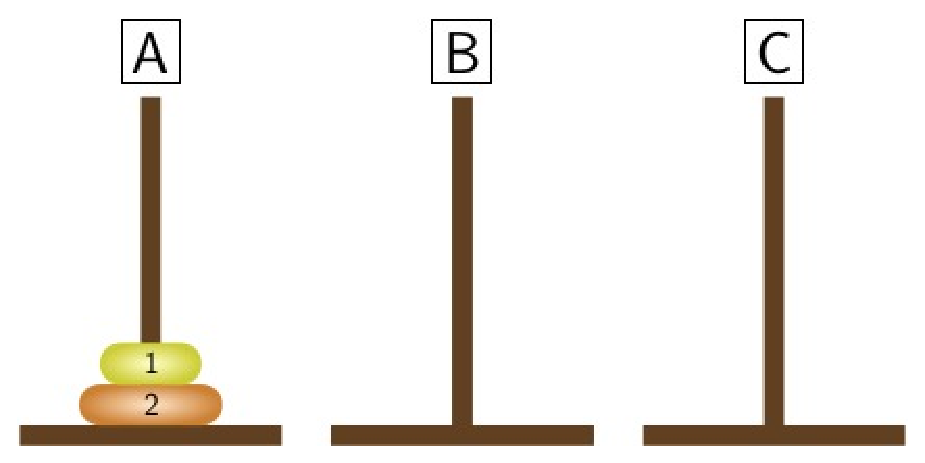
\includegraphics[width=50mm]{./H21}
&
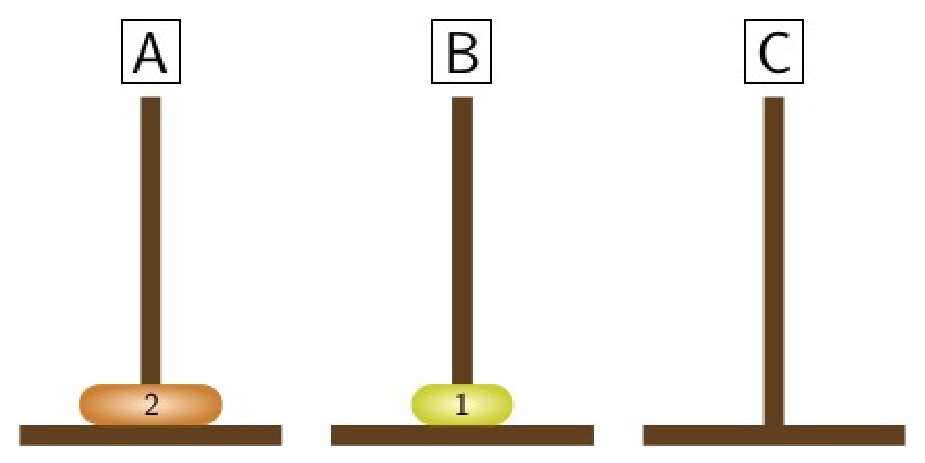
\includegraphics[width=50mm]{./H22}
\end{tabular}
\end{center}
Now we move the disk from peg $A$ to peg $C$.
\begin{center}
\begin{tabular}{l|r}
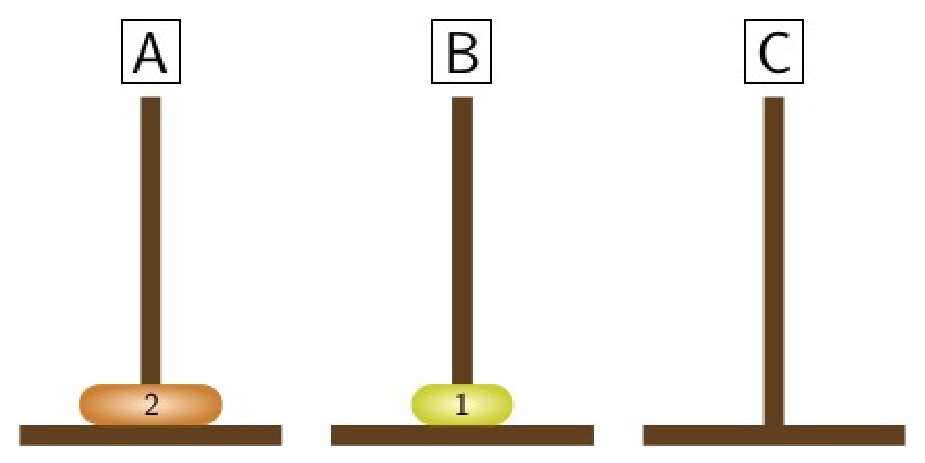
\includegraphics[width=50mm]{./H22}
&
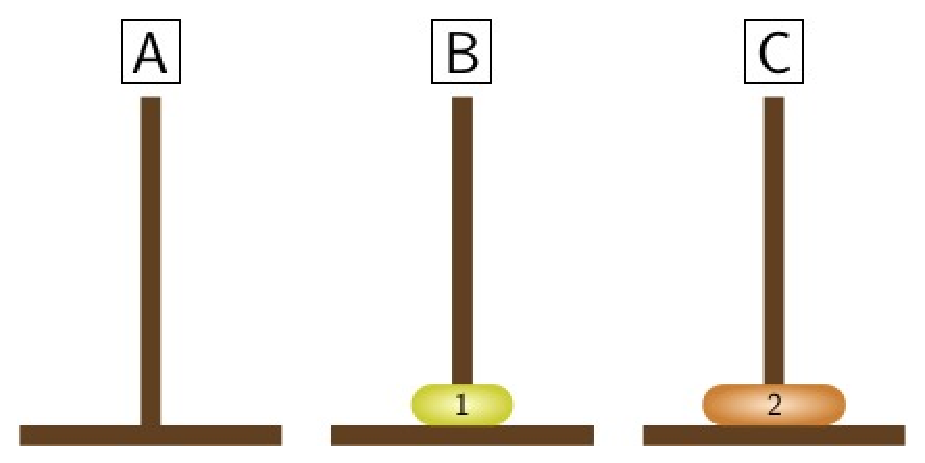
\includegraphics[width=50mm]{./H23}
\end{tabular}
\end{center}
Finally, we move the disk from peg $B$ to peg $C$.
\begin{center}
\begin{tabular}{l|r}
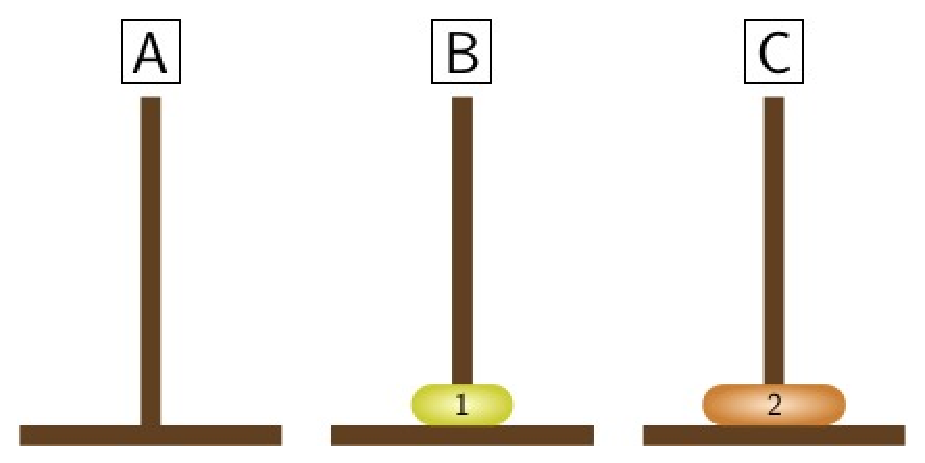
\includegraphics[width=50mm]{./H23}
&
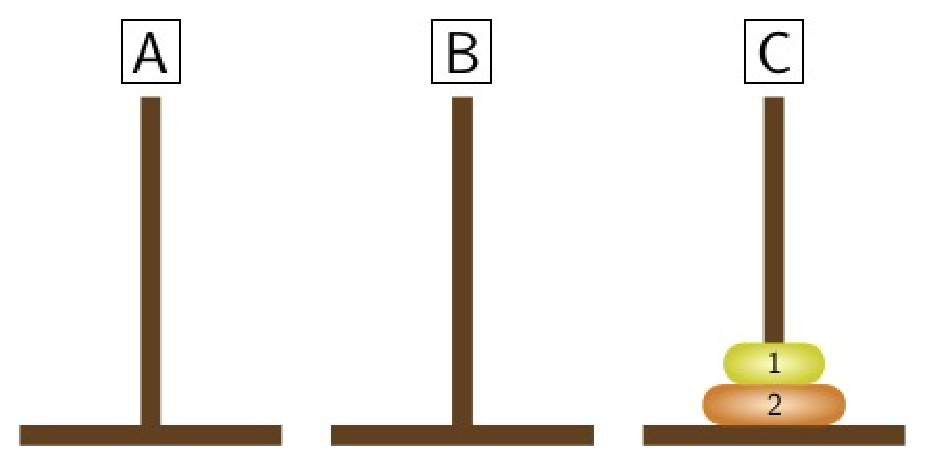
\includegraphics[width=50mm]{./H24}
\end{tabular}
\end{center}
Let us denote by $T_n$ the  minimum number of moves
that will transfer $n$ disks from peg $A$ to peg $C$.
Since no moves are needed to transfer $n=0$ disks, we have that $T_0=0$,
and the previous two examples show that $T_1=1$ and $T_2=3$.
Let us prove that $T_n\leq 2T_{n-1}+1$, that is, there is a solution with $2T_{n-1}+1$ moves.
In $T_{n-1}$ moves we can transfer the $n-1$ smaller disks from peg $A$ to peg $B$. We move the largest
one from peg $A$ to peg $C$ and it remains to move the $n-1$ smallest disks from peg $B$ to peg $C$ and
it can be done in $T_{n-1}$ moves. In total this strategy requires $2T_{n-1}+1$ moves. We only have to show
that $2T_{n-1}+1$ moves are necessary.
If we follow another strategy, then we must move the
largest disk at some point and the $n-1$ smallest disks must be on a single peg (requiring $T_{n-1}$ moves).
After moving the largest disk we must transfer the $n-1$ smallest disks to peg $C$ (requiring another $T_{n-1}$ moves).
It means that $T_n\geq 2T_{n-1}+1$, therefore
$$
T_n=2T_{n-1}+1.
$$
We apply the above strategy to present a minimal solution in case of 3 disks. First we move the 2 smallest disks from peg $A$
to peg $B$. It can be done in $T_2=3$ steps.

STEP 1:
\begin{center}
\begin{tabular}{l|r}
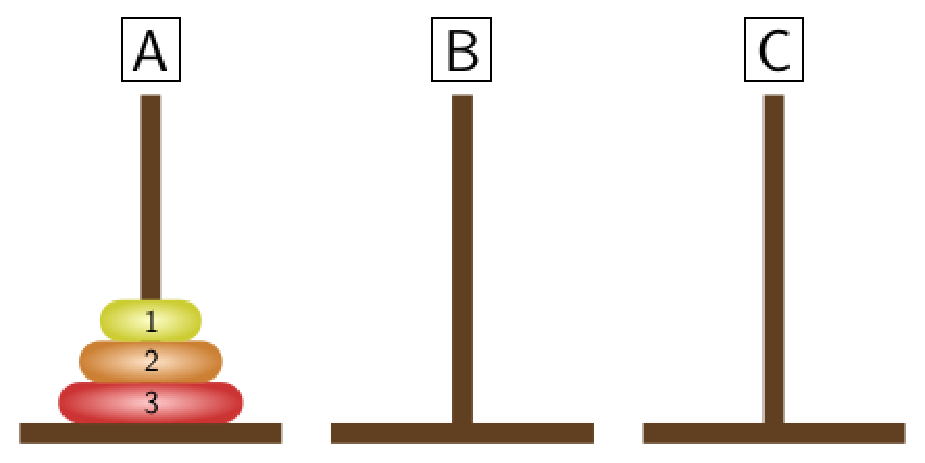
\includegraphics[width=50mm]{./H31-1}
&
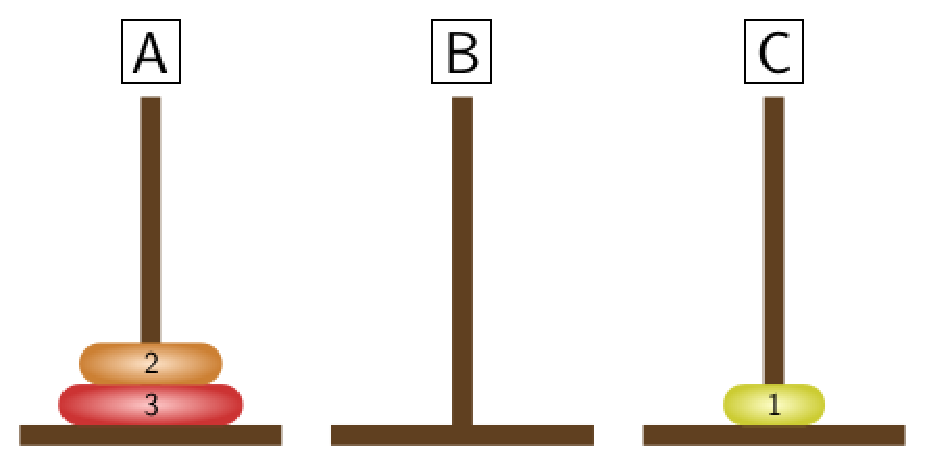
\includegraphics[width=50mm]{./H32-1}
\end{tabular}
\end{center}

STEP 2:
\begin{center}
\begin{tabular}{l|r}
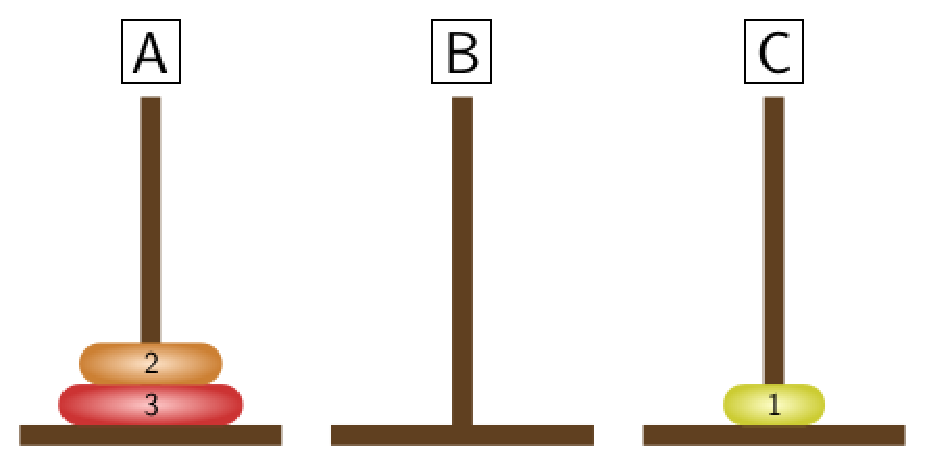
\includegraphics[width=50mm]{./H32-1}
&
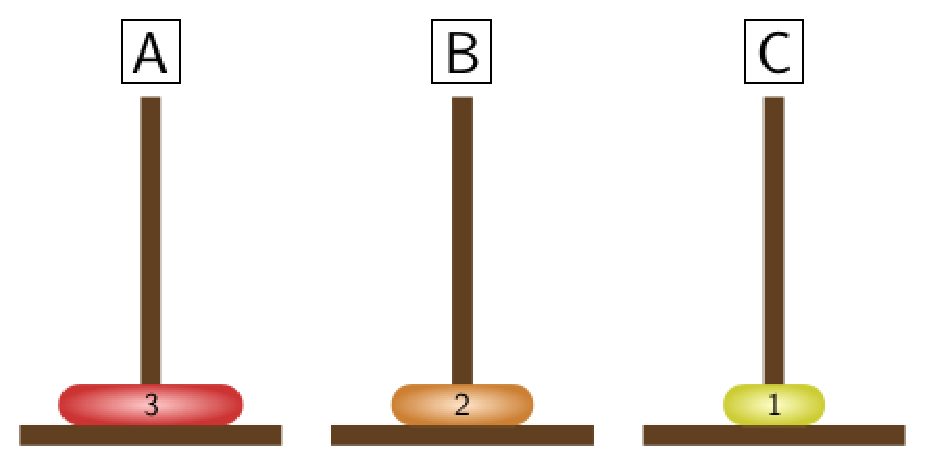
\includegraphics[width=50mm]{./H33-1}
\end{tabular}
\end{center}

STEP 3:
\begin{center}
\begin{tabular}{l|r}
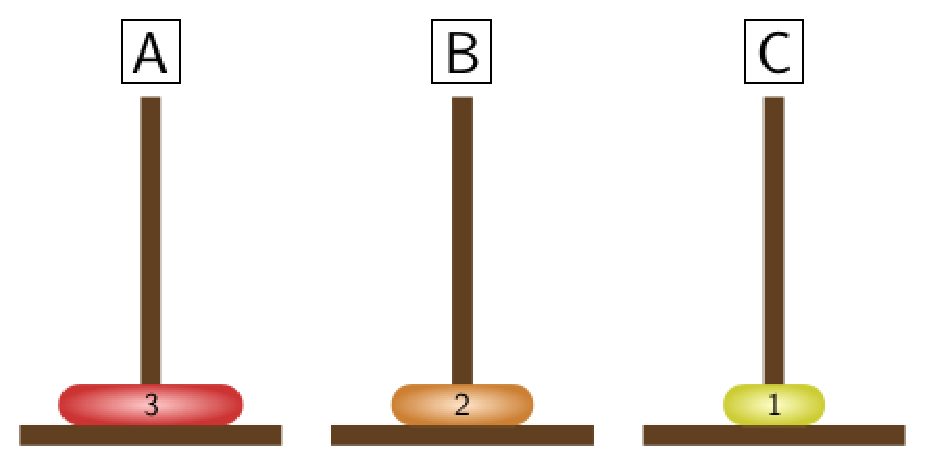
\includegraphics[width=50mm]{./H33-1}
&
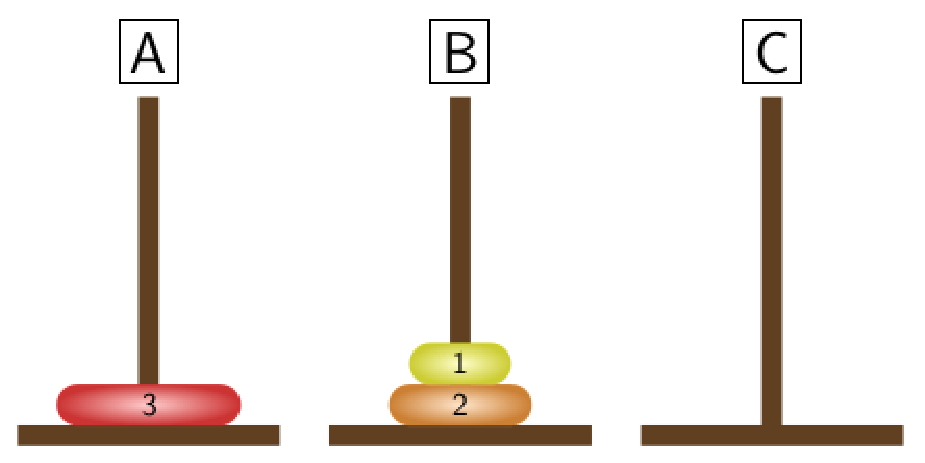
\includegraphics[width=50mm]{./H34-1}
\end{tabular}
\end{center}

Now we can transfer the largest disk to peg $C$.

STEP 4:
\begin{center}
\begin{tabular}{l|r}
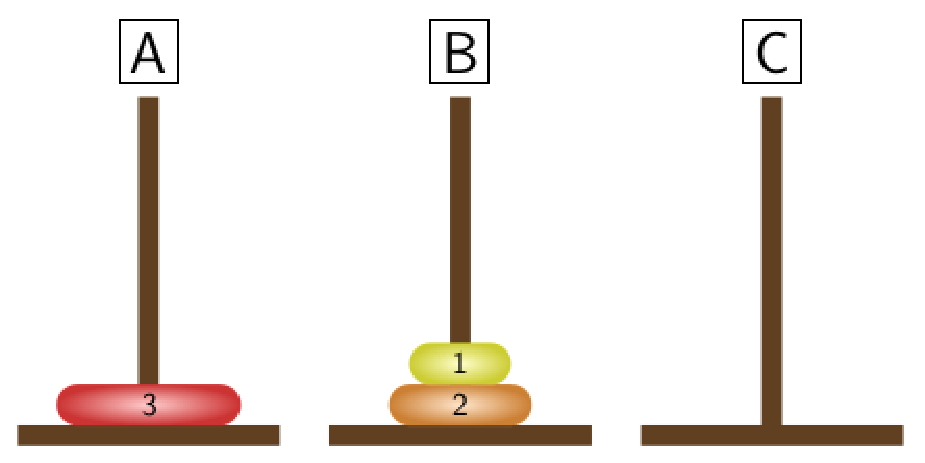
\includegraphics[width=50mm]{./H34-1}
&
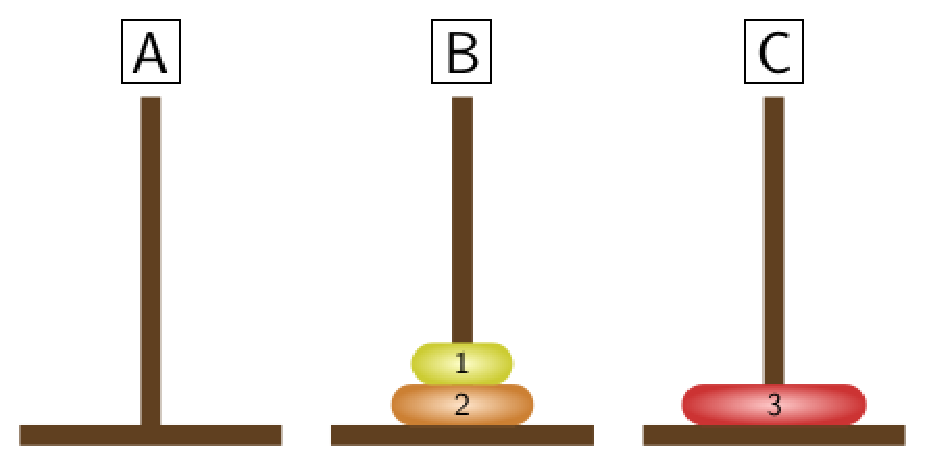
\includegraphics[width=50mm]{./H35-1}
\end{tabular}
\end{center}

It remainst to transfer the 2 smallest disks from peg $B$ to peg $C$, it requires again $T_2=3$ moves.

STEP 5:
\begin{center}
\begin{tabular}{l|r}
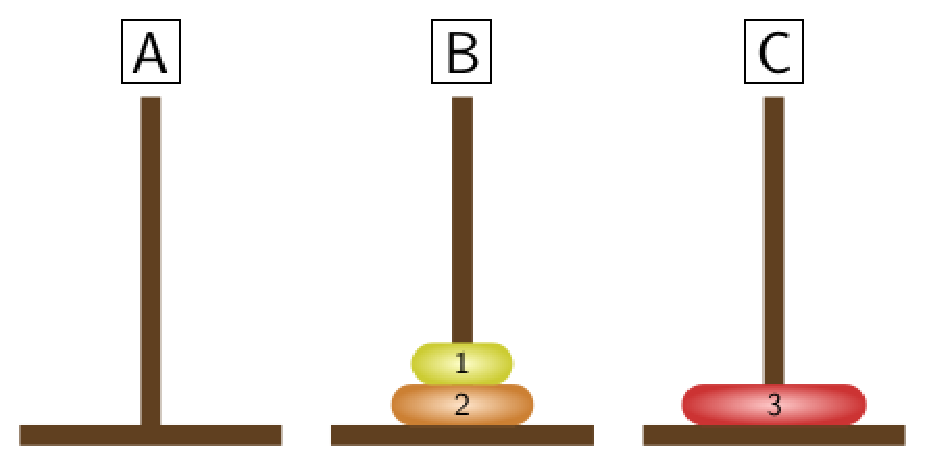
\includegraphics[width=50mm]{./H35-1}
&
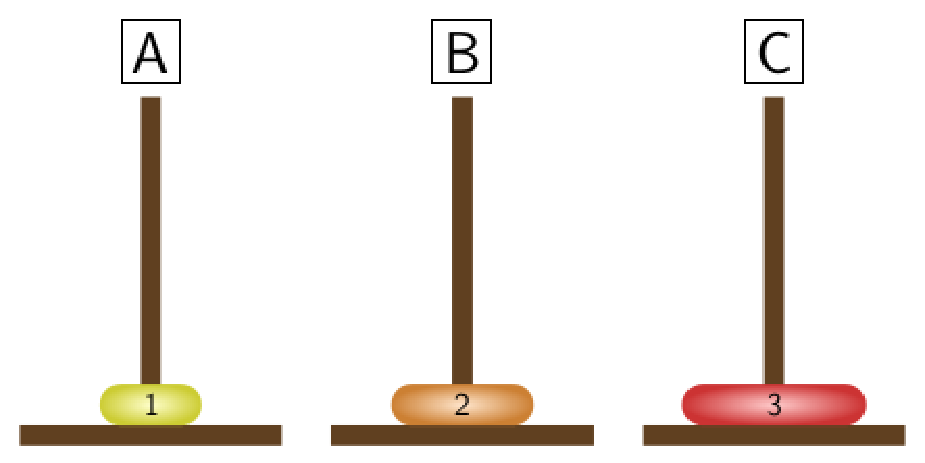
\includegraphics[width=50mm]{./H36-1}
\end{tabular}
\end{center}

STEP 6:
\begin{center}
\begin{tabular}{l|r}
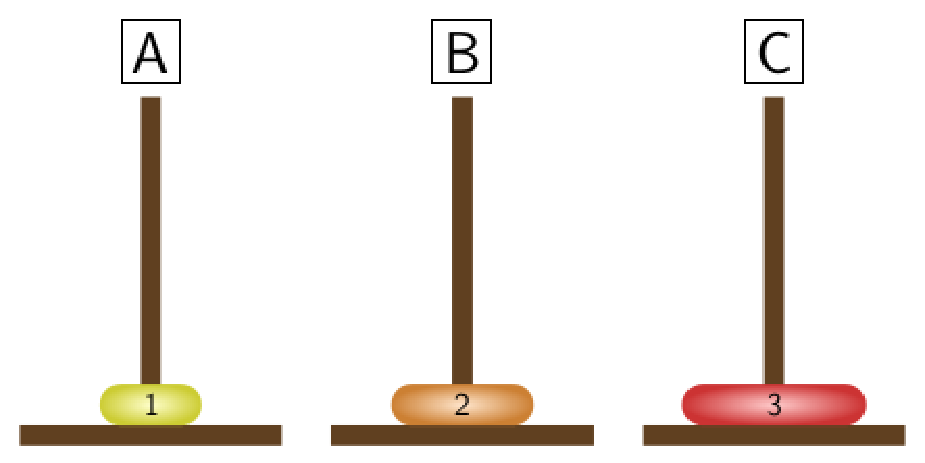
\includegraphics[width=50mm]{./H36-1}
&
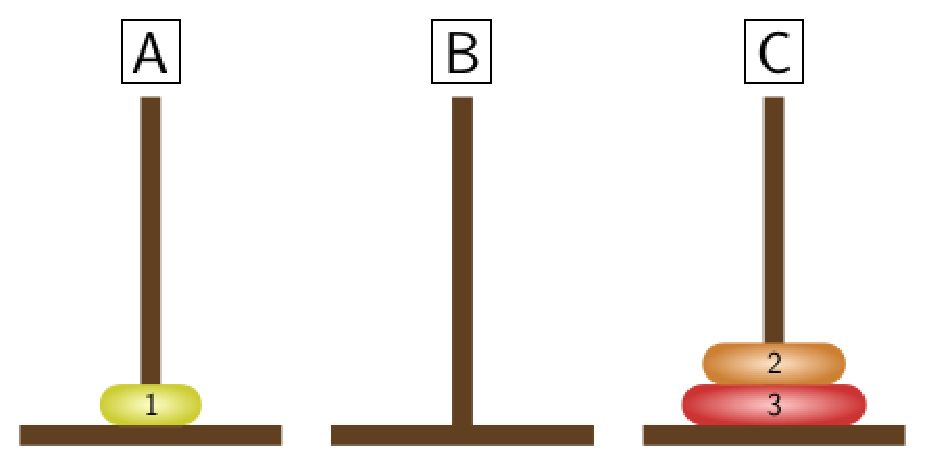
\includegraphics[width=50mm]{./H37-1}
\end{tabular}
\end{center}

STEP 7:
\begin{center}
\begin{tabular}{l|r}
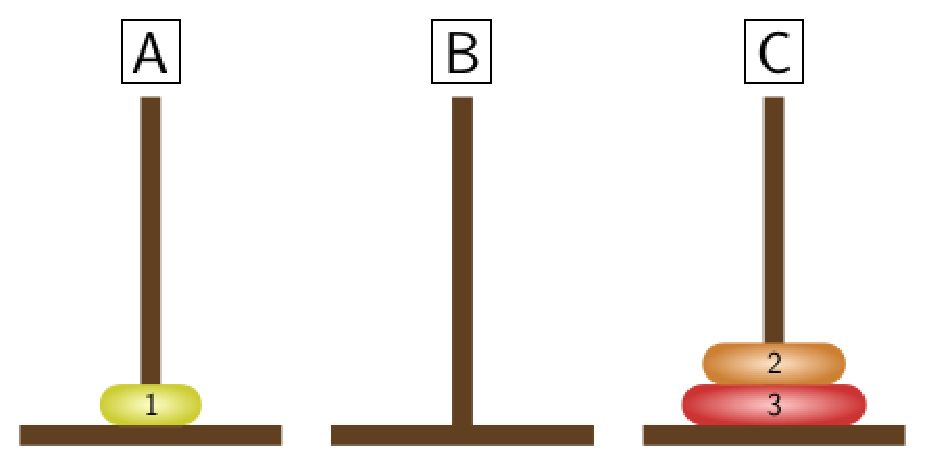
\includegraphics[width=50mm]{./H37-1}
&
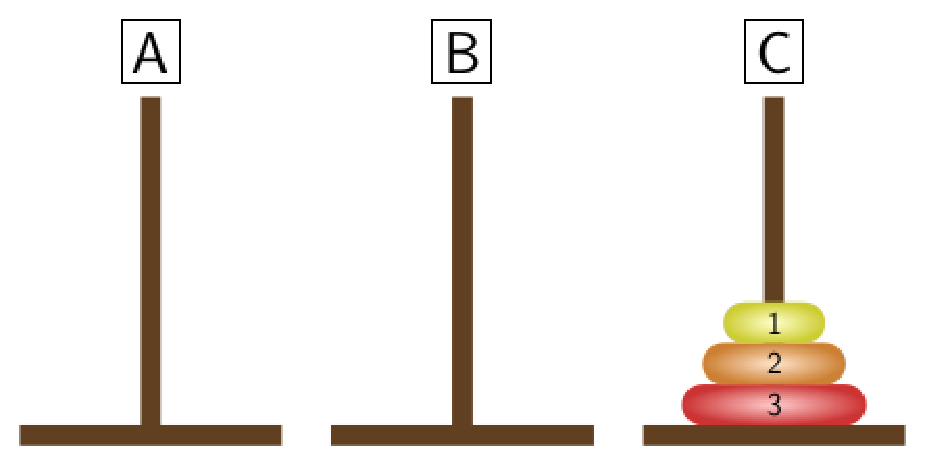
\includegraphics[width=50mm]{./H38-1}
\end{tabular}
\end{center}
Since $T_3=7$ we have found a solution with minimal number of moves.
Having a recurrence relation for the minimal number of moves may help to 
find a nice formula for $T_n$.
The following table contains the first few values of $T_n$.
\begin{center}
\begin{tabular}{|c|c||c|c||c|c|}
\hline
$n$ & $T_n$ & $n$ & $T_n$ & $n$ & $T_n$\\
\hline
0 & 0 & 4 & 15 & 8 & 255\\
\hline
1 & 1 & 5 & 31 & 9 & 511\\
\hline
2 & 3 & 6 & 63 & 10 & 1023\\
\hline
3 & 7 & 7 & 127 & 11 & 2047\\
\hline
\end{tabular}
\end{center}
One can easily observe that these values are 1 less than a power of 2, that is, 
we expect that $T_n=2^n-1$. It can be proved by induction.

\section{Linear recurrence relations of order $k$}
In this section by a sequence we mean an ordered list
$$
\halmaz{a_n}_{n=0}^{\infty},\quad a_n\in S
$$
for some set $S$.
For example 
$$
1,2,4,8,16,32,64,\ldots
$$
is a sequence containing non-negative powers of 2.
\begin{definition}
A sequence $\halmaz{a_n}_{n=0}^{\infty}$  is said to satisfy a \emph{linear recurrence} relation of order $k$ if
$$
a_n=c_{n-1}a_{n-1}+c_{n-2}a_{n-2}+\ldots+c_{n-k}a_{n-k}+b_n,\quad c_{n-k}\neq 0, n\geq k,
$$
where $c_{n-1},\ldots,c_{n-k},b_n$ are some constants. If $b_n=0$, then we say that the sequence
satisfies a \emph{homogeneous linear recurrence} relation of order $k$.
In case of a linear recurrence relation of order $k$ the values of $a_0,a_1,\ldots,a_{k-1}$
are called the \emph{initial values} of the sequence.
\end{definition}
For example the sequence appeared in case of Tower of Hanoi is a sequence of order 1:
\begin{align*}
T_0&=0,\\
T_n&=2T_{n-1}+1 \mbox{ for }n\geq 1.
\end{align*}
\begin{theorem}
Let $\halmaz{a_n}_{n=0}^{\infty}$ be a linear recurrence relation of order 1, that is, 
$$
a_n=ua_{n-1}+v
$$
for some constants $u,v$. If $u=1$, then 
$$
a_n=a_0+nv,
$$
otherwise
$$
a_n=u^na_0+\frac{u^n-1}{u-1}v.
$$
\end{theorem}
\begin{proof}
If $u=1$, then the defining equation simplifies as follows
$$
a_n=a_{n-1}+v.
$$
We prove the statement by induction.
The initial value of the sequence is $a_0$. Using the above formula for $a_n$ we obtain
\begin{align*}
a_1&=a_0+v,\\
a_2&=a_1+v=a_0+2v,\\
a_3&=a_2+v=a_0+3v.
\end{align*}
Hence the statement is clearly true for $n=1,2$ and 3. Assume that the statement is true
for $n=k$, that is, 
$$
a_k=a_0+kv.
$$
The statement for $n=k+1$ is that $a_{k+1}=a_0+(k+1)v$. By the recurrence definition we
have $a_{k+1}=a_{k}+v$. By induction we obtain that 
$$
a_{k+1}=a_0+kv+v=a_0+(k+1)v,
$$
which is the desired result for $n=k+1$.

Now assume that $u\neq 1$. We apply induction again. As in the previous case we compute the first few values of the sequence
\begin{align*}
a_1&=ua_0+v,\\
a_2&=ua_1+v=u^2a_0+uv+v,\\
a_3&=ua_2+v=u^3a_0+u^2v+uv+v.
\end{align*}
It follows that the statement is true if $n=1,2,3$. Assume that the statement is true
for $n=k$, that is, 
$$
a_k=u^ka_0+\frac{u^k-1}{u-1}v.
$$
We need to show that the statement is true for $n=k+1$, so $a_{k+1}=u^{k+1}a_0+\frac{u^{k+1}-1}{u-1}v$.
The recurrence definition yields that
$a_{k+1}=ua_{k}+v$. Using the assumption one has that
$$
a_{k+1}=ua_{k}+v=u\cdot \left(u^ka_0+\frac{u^k-1}{u-1}v\right)+v=u^{k+1}a_0+u\frac{u^k-1}{u-1}v+v.
$$
From the well-known identity $u^m-1=(u-1)\cdot (u^{m-1}+u^{m-2}+\ldots+u+1)$ one gets that 
$$
\frac{u^m-1}{u-1}=u^{m-1}+u^{m-2}+\ldots+u+1
$$
for $u\neq 1$. So we have $u\frac{u^k-1}{u-1}\cdot v+v=(u^k+u^{k-1}+\ldots+u)v+v=(u^k+u^{k-1}+\ldots+u+1)\cdot v$.
Finally we obtain that
$$
a_{k+1}=u^{k+1}a_0+(u^k+u^{k-1}+\ldots+u+1)v=u^{k+1}a_0+\frac{u^{k+1}-1}{u-1}v, 
$$
and the statement follows.
\end{proof}
It is easy to compute an explicit formula for the sequence $T_n$ related to the problem of Tower of Hanoi.
Here $T_n$ is defined as 
\begin{align*}
T_0&=0,\\
T_n&=2T_{n-1}+1 \mbox{ for }n\geq 1,
\end{align*}
that is, $u=2$ and $v=1$. The theorem implies that 
$$
T_n=u^nT_0+\frac{u^n-1}{u-1}v=2^n\cdot 0+\frac{2^n-1}{2-1}\cdot 1=2^n-1.
$$

Consider another example, let $a_n$ be a sequence defined by
\begin{align*}
a_0&=3,\\
a_n&=2a_{n-1}+2 \mbox{ for }n\geq 1.
\end{align*}
We apply the theorem and we have
$$
a_n=2^n\cdot 3+\frac{2^n-1}{2-1}\cdot 2=2^n\cdot 3+2^{n+1}-2=5\cdot 2^n-2.
$$

We have proved a theorem about linear recurrence relations of order 1, given such a recurrence
we are able to provide an explicit formula. What about higher order linear recurrence relations?
To make the presentation simpler we will consider homogeneous linear recurrence relations of order $k$,
where $k\geq 2$. So we study the structure of the recurrence given by
\begin{equation}\label{hlr}
a_n=c_{n-1}a_{n-1}+c_{n-2}a_{n-2}+\ldots+c_{n-k}a_{n-k},\quad c_{n-k}\neq 0, n\geq k,
\end{equation}
where $c_{n-1},\ldots,c_{n-k}$ are some constants.
\begin{theorem}\label{UV}
Assume that $U_n$ and $V_n$ are sequences satisfying \eqref{hlr} and $s,t$ are constants.
The linear combination
$$
W_n=sU_n+tV_n
$$
gives another solution of \eqref{hlr}.
\end{theorem}
\begin{proof}
Since $U_n$ and $V_n$ satisfy \eqref{hlr} we have
\begin{align*}
U_n&=c_{n-1}U_{n-1}+c_{n-2}U_{n-2}+\ldots+c_{n-k}U_{n-k},\\
V_n&=c_{n-1}V_{n-1}+c_{n-2}V_{n-2}+\ldots+c_{n-k}V_{n-k}.
\end{align*}
Substituting these formulas into the definition of $W_n$ we get
\begin{align*}
W_n=&s(c_{n-1}U_{n-1}+c_{n-2}U_{n-2}+\ldots+c_{n-k}U_{n-k})+\\
&t(c_{n-1}V_{n-1}+c_{n-2}V_{n-2}+\ldots+c_{n-k}V_{n-k})=\\
&c_{n-1}(sU_{n-1}+tV_{n-1})+c_{n-2}(sU_{n-2}+tV_{n-2})+\ldots+\\
&+c_{n-k}(sU_{n-k}+tV_{n-k})=\\
&c_{n-1}W_{n-1}+c_{n-2}W_{n-2}+\ldots+c_{n-k}W_{n-k}.
\end{align*}
It turned out that $W_n$ is also a solution of \eqref{hlr}.
\end{proof}
The previous theorem suggests a strategy to determine explicit formula
for higher order linear homogeneous recurrence relations. First we look for solutions
of the concrete recurrence relation, then we consider linear combinations of them
and we try to fix the constants in such a way that the initial values of the given sequence
are the same as in case of the sequence obtained by linear combination. What kind of solutions
should we look for? Here we need some numerical experiences. Consider the example
\begin{align*}
a_0&=2,\\
a_1&=2,\\
a_n&=2a_{n-1}+3a_{n-2},\quad n\geq 2.
\end{align*}
The above sequence is a homogeneous linear recurrence sequence of order $2$.
We can easily compute the first few elements of the sequence, $a_2=10, a_3=26, a_4=82$.
Let us consider the ratio of consecutive elements of the sequence.
\begin{center}
\begin{tabular}{|c|c||c|c|}
\hline
$n$ & $\frac{a_n}{a_{n-1}}$ & $n$ & $\frac{a_n}{a_{n-1}}$\\
\hline
1 & $1$ & 5 & $\approx 2.951$\\
\hline
2 & $5$ & 6 & $\approx 3.017$\\
\hline
3 & $2.6$ & 7 & $\approx 2.995$\\
\hline
4 & $\approx 3.154$ & 8 & $\approx 3.002$\\
\hline
\end{tabular}
\end{center}
The ratios are very close to a constant, in this case very close to 3 for $n\in\halmaz{4,5,6,7,8}$.
At the beginning of this chapter we studied sequences for which the ratio of consecutive elements
is a constant, these are geometric progressions. Let us look for geometric progressions satisfying
the same recurrence relation as $a_n$. If $g_n$ is a sequence given by
the formula
$$
g_n=rg_{n-1},
$$
where $r$ is the common ratio of the sequence with initial value $g_0$, then we have that 
$g_n=g_0r^n$. That is, $g_n$ is a geometric progression. Let us assume that for some initial
value $g_0$ and for some $r$ the progression satisfies the same recurrence relation as $a_n$.
Now we obtain
$$
g_n=2g_{n-1}+3g_{n-2}.
$$
It follows that
$$
g_0r^n=2g_0r^{n-1}+3g_0r^{n-2}.
$$
The constant zero progression is not useful for our purposes we assume that $g_0\neq 0$ and $r\neq 0$.
After dividing by $g_0r^{n-2}$ we get
$$
r^2=2r+3.
$$
If there is such a progression, then $r$ is a root of the quadratic polynomial $r^2-2r-3$.
One can determine the roots by the well-known formula, which is in our case
$$
\frac{2\pm\sqrt{4-4(-3)}}{2}.
$$
That is, the roots are $3$ and $-1$. We have two different solutions of the recurrence relation
and Theorem~\ref{UV} implies that linear combinations of these two solutions yield another solutions.
Let us consider the sequence $W_n=s3^n+t(-1)^n$. We should fix $s,t$ in such a way that 
\begin{align*}
&W_0=a_0=2,\\
&W_1=a_1=2.
\end{align*}
We get a system of equations in two unknowns
\begin{align*}
W_0=2&\Rightarrow s\cdot 3^0+t\cdot (-1)^0=2,\\
W_1=2&\Rightarrow s\cdot 3^1+t\cdot (-1)^1=2.
\end{align*}
The first equation implies that $t=2-s$. The second equation can be written as $3s+(2-s)(-1)=2$, that is, $4s=4$ and we get that $s=1,t=1$.
Now we have a sequence $W_n=3^n+(-1)^n$ which satisfies the appropriate recurrence relation and has the same initial values as $a_n$.
Thus $W_n=a_n$. In this way we obtained an explicit formula for the recurrence sequence $a_n$ given by
$$
3^n+(-1)^n.
$$
We may try to apply the above method to determine an explicit formula for the famous Fibonacci sequence:
\begin{align*}
F_0&=0,\\
F_1&=1,\\
F_n&=F_{n-1}+F_{n-2},\quad n\geq 2.
\end{align*}
Let $g_n$ be a geometric progression such that $g_n=g_0r^n$ for some $g_0$ and $r$.
Assume that $g_n$ satisfies the recurrence relation. It follows that
$$
r^2=r+1.
$$
The two roots of this quadratic polynomial are
$$
\frac{1-\sqrt{5}}{2}\quad\mbox{ and }\quad\frac{1+\sqrt{5}}{2}.
$$
Let $W_n$ be a linear combination of the appropriate geometric progressions, that is, 
$$
W_n=s\cdot \left(\frac{1-\sqrt{5}}{2}\right)^n+t\cdot \left(\frac{1+\sqrt{5}}{2}\right)^n.
$$
It remains to find $s$ and $t$ for which
\begin{align*}
&W_0=F_0=0,\\
&W_1=F_1=1.
\end{align*}
The above equations imply that
\begin{align*}
s+t&=0\\
s\cdot \left(\frac{1-\sqrt{5}}{2}\right)+t\cdot \left(\frac{1+\sqrt{5}}{2}\right)&=1.
\end{align*}
We immediately get that $t=-s$. Therefore
$$
s\cdot \left(\frac{1-\sqrt{5}}{2}\right)-s\cdot \left(\frac{1+\sqrt{5}}{2}\right)=1.
$$
The latter equation yields that $s=\frac{-\sqrt{5}}{5}$, so  $t=\frac{\sqrt{5}}{5}$.
The explicit formula in case of the Fibonacci sequence is
$$
F_n=\frac{-\sqrt{5}}{5}\cdot \left(\frac{1-\sqrt{5}}{2}\right)^n+\frac{\sqrt{5}}{5}\cdot \left(\frac{1+\sqrt{5}}{2}\right)^n.
$$
Let us see if the previous argument works for homogeneous linear recurrence sequence of order greater than 2.
We define $a_n$ as
\begin{align*}
a_0&=5,\\
a_1&=-3,\\
a_2&=11,\\
a_n&=-a_{n-1}+4a_{n-2}+4a_{n-3},\quad n\geq 3.
\end{align*}
The sequence $a_n$ is a homogeneous linear recurrence sequence of order 3, since $a_n$ depends on 
the previous 3 elements of the sequence. We try to find a geometric progression $g_n=g_0r^n$ satisfying
the above recurrence
$$
g_0r^n=-g_0r^{n-1}+4g_0r^{n-2}+4g_0r^{n-3}.
$$
Again we exclude the case $g_0r=0$, so we may simplify the equation by $g_0r^{n-3}$.
So we obtain
$$
r^3+r^2-4r-4=0.
$$
This time we have a cubic polynomial and finding the roots of a cubic is more difficult than determining
the roots of a quadratic polynomial. We may try to find some special roots e.g.\ integral roots. 
To find integral roots we can rewrite the equation in the form
$$
r\cdot (r^2+r-4)=4.
$$
If $r$ is an integer, then the expression on the left-hand side is a multiple of two integers. The multiple
of two integers is equal to 4, that is, we have only a few possibilities since $r$ has to divide 4. That
is $r\in\halmaz{-4,-2,-1,1,2,4}$. Evaluate the cubic polynomial at these values:
\begin{center}
\begin{tabular}{|c|c|}
\hline
$r$ & $r^3+r^2-4r-4$\\
\hline
-4 & -36\\
\hline
-2 & 0\\
\hline
-1 & 0\\
\hline
 1 & -6\\
 \hline
 2 & 0\\
 \hline
 4 & 60\\
 \hline
\end{tabular}
\end{center}
We are lucky, there are 3 integral roots: $-2,-1$ and 2. It means by Theorem~\ref{UV} that any linear combinations
of the geometric progressions $(-2)^n, (-1)^n$ and $2^n$ will satisfy the same recurrence relation as $a_n$.
Now define $W_n=s(-2)^n+t(-1)^n+u2^n$. Our task is to fix $s,t$ and $u$ such that
\begin{align*}
&W_0=a_0=5,\\
&W_1=a_1=-3,\\
&W_2=a_2=11.
\end{align*}
These equations yield a system of equations in three unknowns.
\begin{align*}
s+t+u&=5\\
-2s-t+2u&=-3\\
4s+t+4u&=11.
\end{align*}
We can eliminate $s$ and $u$ using the first and the third equations. To do so we multiply the first equation by 4:
\begin{align*}
4s+4t+4u&=20\\
-2s-t+2u&=-3\\
4s+t+4u&=11.
\end{align*}
We subtract the third equation from the first one and we get
$$
3t=9,
$$
that is, $t=3$. The system of equations can be simplified now:
\begin{align*}
s+u&=2\\
-2s+2u&=0.
\end{align*}
The second equation implies that $s=u$, so from the first equation we have that $s=u=1$.
The explicit formula for the sequence $a_n$ is
$$
(-2)^n+3\cdot (-1)^n+2^n.
$$

We remark that the previous argument does not work if we have a root with multiplicity greater than 1.
Without providing the details of the theory we note that it is also possible to handle such cases. For example
assume that a linear recurrence of order 2 is given and the corresponding quadratic polynomial has a double root $r$.
We have that $r^n$ and $nr^n$ are solutions of the same recurrence. In general, if we have a linear recurrence of order $k$
and the corresponding polynomial has a root $r$ with multiplicity $m$, then 
$$
r^n,\quad nr^n,\ldots n^{m-1}r^n
$$
are solutions of the same recurrence.
Let us consider an example.
\begin{align*}
u_0&=4,\\
u_1&=-1,\\
u_2&=-1,\\
u_3&=-43,\\
u_n&=5u_{n-1}-6u_{n-2}-4u_{n-3}+8u_{n-4},\quad n\geq 4.
\end{align*}
The corresponding quartic polynomial $r^4-5r^3+6r^2+4r-8$ can be written as $(r+1)(r-2)^3$,
that is, $-1$ is a simple root and 2 is a root with multiplicity 3. Therefore we define $W_n$ as
$$
s\cdot (-1)^n+t\cdot 2^n+xn\cdot 2^n+yn^2\cdot 2^n.
$$
Then we obtain four equations in four unknowns
\begin{align*}
s+t&=4\\
-s+2t+2x+2y&=-1\\
s+4t+8x+16y&=-1\\
-s+8t+24x+72y&=-43.
\end{align*}
We get that $s=4-t$, hence
\begin{align*}
3t+2x+2y&=3\\
3t+8x+16y&=-5\\
9t+24x+72y&=-39.
\end{align*}
Using the first equation we can eliminate $t$ from the second and the third equations.
\begin{align*}
6x+14y&=-8\\
18x+66y&=-48.
\end{align*}
The above system has the solution $x=1, y=-1$. We get that $t=1$ and $s=3$.
Thus
$$
u_n=3\cdot (-1)^n+2^n+n\cdot 2^n-n^2\cdot 2^n.
$$
As an application we deal with an inverse problem, let us be given the sequence
$$
u_n=\left(\frac{3-\sqrt{33}}{2}\right)^n+\left(\frac{3+\sqrt{33}}{2}\right)^n,\quad n\geq 0.
$$
Our statement is that $u_n$ is an integer sequence and 3 divides $u_n$ for $n\geq 1$. This statement
can be proved by induction (Exercise~\ref{induction-6}), but now we apply the theory of linear recurrence sequences. We are given an
explicit formula and we would like to determine a linear recurrence sequence which has the same closed-form
solution. It is easy to see that $u_0=2$ and $u_1=3$. If we have an appropriate recurrence, then $\frac{3-\sqrt{33}}{2}$
and $\frac{3+\sqrt{33}}{2}$ are roots of some quadratic polynomial:
$$
\left(r-\frac{3-\sqrt{33}}{2}\right)\cdot \left(r-\frac{3+\sqrt{33}}{2}\right)=r^2-3r-6.
$$
From this polynomial we have the following recurrence relation $u_n=3u_{n-1}+6u_{n-2}$.
That is, we have a recurrence sequence
\begin{align*}
u_0&=2,\\
u_1&=3,\\
u_n&=3u_{n-1}+6u_{n-2}=3(u_{n-1}+2u_{n-2}).
\end{align*}
Since $u_0$ and $u_1$ are integers and $u_{n-1},u_{n-2}$ have integral coefficients in the recurrence relation, the sequence $u_n$
is an integral sequence. It is clear that $u_1=3$ is divisible by 3 and similarly $u_n=3(u_{n-1}+2u_{n-2})$ is a multiple of 3.

\begin{exercise}\label{seq-ex-1}
Find the shortest sequence of moves that transfers a tower of 4
disks from peg $A$ to peg $C$.
\end{exercise}

\begin{exercise}\label{seq-ex-2}
Find a closed-form formula for the following sequence defined by:
$$
a_n=7a_{n-1}-10a_{n-2}\quad\mbox{ for }n\geq 2\quad\mbox{ and }a_0=0,a_1=2.
$$
\end{exercise}

\begin{exercise}\label{seq-ex-3}
Find an explicit formula for the following sequence defined by:
$$
a_n=4a_{n-1}-3a_{n-2}\quad\mbox{ for }n\geq 2\quad\mbox{ and }a_0=1,a_1=13.
$$
\end{exercise}

\begin{exercise}\label{seq-ex-4}
Find a closed-form formula for the following sequence defined by:
$$
a_n=-2a_{n-1}+a_{n-2}+2a_{n-3}\quad\mbox{ for }n\geq 3\quad\mbox{ and }a_0=0,a_1=1,a_2=2.
$$
\end{exercise}

\begin{exercise}\label{seq-ex-5}
Find an explicit formula for the following sequence defined by:
$$
a_n=6a_{n-1}-11a_{n-2}+6a_{n-3}\quad\mbox{ for }n\geq 3\quad\mbox{ and }a_0=0,a_1=0,a_2=1.
$$
\end{exercise}

\begin{exercise}\label{seq-ex-6}
Find a closed-form formula for the following sequence defined by:
$$
a_n=4a_{n-1}-4a_{n-2}\quad\mbox{ for }n\geq 2\quad\mbox{ and }a_0=-1,a_1=0.
$$
\end{exercise}

\begin{exercise}\label{seq-ex-7}
Find an explicit formula for the following sequence defined by:
$$
a_n=5a_{n-1}-3a_{n-2}-9a_{n-3}\quad\mbox{ for }n\geq 3\quad\mbox{ and }a_0=3,a_1=4,a_2=29.
$$
\end{exercise}

\begin{exercise}\label{seq-ex-8}
Prove that the sequence defined by
$$
u_n=\left(\frac{5-3\sqrt{5}}{2}\right)^n+\left(\frac{5+3\sqrt{5}}{2}\right)^n,\quad n\geq 0
$$
contains only integers and $u_n$ is divisible by 5 if $n\geq 1$.
\end{exercise}

\begin{exercise}\label{seq-ex-9}
Prove that the sequence defined by
$$
(4-\sqrt{2})^n+(4+\sqrt{2})^n,\quad n\geq 0
$$
contains only integers divisible by 2.
\end{exercise}
